% Options for packages loaded elsewhere
\PassOptionsToPackage{unicode}{hyperref}
\PassOptionsToPackage{hyphens}{url}
\PassOptionsToPackage{dvipsnames,svgnames,x11names}{xcolor}
%
\documentclass[
  man,floatsintext]{apa6}
\usepackage{amsmath,amssymb}
\usepackage{lmodern}
\usepackage{iftex}
\ifPDFTeX
  \usepackage[T1]{fontenc}
  \usepackage[utf8]{inputenc}
  \usepackage{textcomp} % provide euro and other symbols
\else % if luatex or xetex
  \usepackage{unicode-math}
  \defaultfontfeatures{Scale=MatchLowercase}
  \defaultfontfeatures[\rmfamily]{Ligatures=TeX,Scale=1}
\fi
% Use upquote if available, for straight quotes in verbatim environments
\IfFileExists{upquote.sty}{\usepackage{upquote}}{}
\IfFileExists{microtype.sty}{% use microtype if available
  \usepackage[]{microtype}
  \UseMicrotypeSet[protrusion]{basicmath} % disable protrusion for tt fonts
}{}
\makeatletter
\@ifundefined{KOMAClassName}{% if non-KOMA class
  \IfFileExists{parskip.sty}{%
    \usepackage{parskip}
  }{% else
    \setlength{\parindent}{0pt}
    \setlength{\parskip}{6pt plus 2pt minus 1pt}}
}{% if KOMA class
  \KOMAoptions{parskip=half}}
\makeatother
\usepackage{xcolor}
\IfFileExists{xurl.sty}{\usepackage{xurl}}{} % add URL line breaks if available
\IfFileExists{bookmark.sty}{\usepackage{bookmark}}{\usepackage{hyperref}}
\hypersetup{
  pdftitle={Getting a Step Ahead: Using the Regularized Horseshoe Prior to Select Cross-Loadings in Bayesian CFA},
  pdflang={en-EN},
  colorlinks=true,
  linkcolor={Maroon},
  filecolor={Maroon},
  citecolor={Blue},
  urlcolor={blue},
  pdfcreator={LaTeX via pandoc}}
\urlstyle{same} % disable monospaced font for URLs
\usepackage{graphicx}
\makeatletter
\def\maxwidth{\ifdim\Gin@nat@width>\linewidth\linewidth\else\Gin@nat@width\fi}
\def\maxheight{\ifdim\Gin@nat@height>\textheight\textheight\else\Gin@nat@height\fi}
\makeatother
% Scale images if necessary, so that they will not overflow the page
% margins by default, and it is still possible to overwrite the defaults
% using explicit options in \includegraphics[width, height, ...]{}
\setkeys{Gin}{width=\maxwidth,height=\maxheight,keepaspectratio}
% Set default figure placement to htbp
\makeatletter
\def\fps@figure{htbp}
\makeatother
\setlength{\emergencystretch}{3em} % prevent overfull lines
\providecommand{\tightlist}{%
  \setlength{\itemsep}{0pt}\setlength{\parskip}{0pt}}
\setcounter{secnumdepth}{-\maxdimen} % remove section numbering
% Make \paragraph and \subparagraph free-standing
\ifx\paragraph\undefined\else
  \let\oldparagraph\paragraph
  \renewcommand{\paragraph}[1]{\oldparagraph{#1}\mbox{}}
\fi
\ifx\subparagraph\undefined\else
  \let\oldsubparagraph\subparagraph
  \renewcommand{\subparagraph}[1]{\oldsubparagraph{#1}\mbox{}}
\fi
\newlength{\cslhangindent}
\setlength{\cslhangindent}{1.5em}
\newlength{\csllabelwidth}
\setlength{\csllabelwidth}{3em}
\newlength{\cslentryspacingunit} % times entry-spacing
\setlength{\cslentryspacingunit}{\parskip}
\newenvironment{CSLReferences}[2] % #1 hanging-ident, #2 entry spacing
 {% don't indent paragraphs
  \setlength{\parindent}{0pt}
  % turn on hanging indent if param 1 is 1
  \ifodd #1
  \let\oldpar\par
  \def\par{\hangindent=\cslhangindent\oldpar}
  \fi
  % set entry spacing
  \setlength{\parskip}{#2\cslentryspacingunit}
 }%
 {}
\usepackage{calc}
\newcommand{\CSLBlock}[1]{#1\hfill\break}
\newcommand{\CSLLeftMargin}[1]{\parbox[t]{\csllabelwidth}{#1}}
\newcommand{\CSLRightInline}[1]{\parbox[t]{\linewidth - \csllabelwidth}{#1}\break}
\newcommand{\CSLIndent}[1]{\hspace{\cslhangindent}#1}
\ifLuaTeX
\usepackage[bidi=basic]{babel}
\else
\usepackage[bidi=default]{babel}
\fi
\babelprovide[main,import]{english}
% get rid of language-specific shorthands (see #6817):
\let\LanguageShortHands\languageshorthands
\def\languageshorthands#1{}
% This preamble allows to remove the redundant title page from papaja's output.pdf
\usepackage{atbegshi}% http://ctan.org/pkg/atbegshi
\AtBeginDocument{\AtBeginShipoutNext{\AtBeginShipoutDiscard}}
% Manuscript styling
\usepackage{upgreek}
\captionsetup{font=singlespacing,justification=justified}

% Table formatting
\usepackage{longtable}
\usepackage{lscape}
% \usepackage[counterclockwise]{rotating}   % Landscape page setup for large tables
\usepackage{multirow}		% Table styling
\usepackage{tabularx}		% Control Column width
\usepackage[flushleft]{threeparttable}	% Allows for three part tables with a specified notes section
\usepackage{threeparttablex}            % Lets threeparttable work with longtable

% Create new environments so endfloat can handle them
% \newenvironment{ltable}
%   {\begin{landscape}\centering\begin{threeparttable}}
%   {\end{threeparttable}\end{landscape}}
\newenvironment{lltable}{\begin{landscape}\centering\begin{ThreePartTable}}{\end{ThreePartTable}\end{landscape}}

% Enables adjusting longtable caption width to table width
% Solution found at http://golatex.de/longtable-mit-caption-so-breit-wie-die-tabelle-t15767.html
\makeatletter
\newcommand\LastLTentrywidth{1em}
\newlength\longtablewidth
\setlength{\longtablewidth}{1in}
\newcommand{\getlongtablewidth}{\begingroup \ifcsname LT@\roman{LT@tables}\endcsname \global\longtablewidth=0pt \renewcommand{\LT@entry}[2]{\global\advance\longtablewidth by ##2\relax\gdef\LastLTentrywidth{##2}}\@nameuse{LT@\roman{LT@tables}} \fi \endgroup}

% \setlength{\parindent}{0.5in}
% \setlength{\parskip}{0pt plus 0pt minus 0pt}

% \usepackage{etoolbox}
\makeatletter
\patchcmd{\HyOrg@maketitle}
  {\section{\normalfont\normalsize\abstractname}}
  {\section*{\normalfont\normalsize\abstractname}}
  {}{\typeout{Failed to patch abstract.}}
\patchcmd{\HyOrg@maketitle}
  {\section{\protect\normalfont{\@title}}}
  {\section*{\protect\normalfont{\@title}}}
  {}{\typeout{Failed to patch title.}}
\makeatother
\shorttitle{Getting a Step Ahead: Using the Regularized Horseshoe Prior to Select Cross-Loadings in Bayesian CFA}
\keywords{\newline\indent Word count: X}
\DeclareDelayedFloatFlavor{ThreePartTable}{table}
\DeclareDelayedFloatFlavor{lltable}{table}
\DeclareDelayedFloatFlavor*{longtable}{table}
\makeatletter
\renewcommand{\efloat@iwrite}[1]{\immediate\expandafter\protected@write\csname efloat@post#1\endcsname{}}
\makeatother
\usepackage{csquotes}
\ifLuaTeX
  \usepackage{selnolig}  % disable illegal ligatures
\fi

\title{Getting a Step Ahead: Using the Regularized Horseshoe Prior to Select Cross-Loadings in Bayesian CFA}
\author{\phantom{0}}
\date{}


\affiliation{\phantom{0}}

\begin{document}
\maketitle

% move text to bottom of page
\vfill
Research Report\\
Michael Koch (6412157)\\
Methodology and Statistics for the Behavioral, Biomedical, and Social Sciences \\
Supervisor: Dr. Sara van Erp \\ 
Email: j.m.b.koch@students.uu.nl \\
Word Count: 2469 \\
Intented Journal of Publication: Structural Equation Modeling \\

% make page numbers start from second page 
\pagenumbering{arabic}
\setcounter{page}{0}
\thispagestyle{empty}
% make page numbers from second page 
\pagestyle{plain}

\clearpage

The art of statistical modeling revolves around coming up with an appropriate simplification, a \emph{model}, of a true \emph{data-generating process}. Hereby, a fundamental trade-off between model simplicity and model complexity arises, that is mostly known as \emph{bias-variance trade-off}. Simple models with few parameters have high bias, meaning that they deviate substantially from the true data-generating process. However, these models have low variance, hence they generalize well to other datasets from the same population. Moreover, simple models are easily identified (estimatable with the information available in the data) and easy to interpret. Complex models with large numbers of parameters tend to have low bias and high variance. Consequently, complex models are prone to over-fitting, i.e.~picking up patterns that are only relevant in the dataset at hand, but do not generalize well to other datasets. Moreover, complex models can be cumbersome to interpret and often a large number of observations is required to estimate them (Cox, 2006; James, Witten, Hastie, \& Tibshirani, 2021).

\hypertarget{regularization}{%
\subsection{Regularization}\label{regularization}}

A classic way of dealing with the bias-variance trade-off is \emph{regularization} (Hastie, Tibshirani, \& Wainwright, 2015). At its core regularization entails willingly adding some bias to the model to reduce its variance. This helps to ensure that the model becomes easier to interpret and more generalizable. In a frequentist context, regularization is achieved by adding a penality term to the cost function of a model. Such penalty ensures that model parameters that are deemed irrelevant, e.g.~small regression coefficients in a regression model with a large number of predictors, are shrunken to (or towards) zero. In a Bayesian context, the same is achieved by setting a so-called shrinkage-prior for the parameters (Van Erp, Oberski, \& Mulder, 2019). The well-known ridge- (Hoerl \& Kennard, 2000) and lasso-penalization (Tibshirani, 1996) in regression correspond to setting a ridge-prior (Hsiang, 1975) or a Laplace-prior (Park \& Casella, 2008) for regression coefficients respectively.

\hypertarget{simple-structure-in-cfa}{%
\subsection{Simple Structure in CFA}\label{simple-structure-in-cfa}}

In Confirmatory factor analysis (CFA, Bollen, 1989), an essential tool for modeling measurement structures, it is common practice to deal with the bias-variance trade-off in a brute-force manner, by imposing a so-called simple structure. Here, cross-loadings, factor loadings that relate items to factors that they theoretically do not belong to, are fixed to zero to yield an identified and interpretable model. This often leads to poor model fit, which forces researchers to free some cross-loadings after the fact based on empirical grounds (modification indices) to improve fit. This procedure is flawed, as it risks capitalization on chance and thereby over-fitting, hence ending up with a model that does not generalize well to other datasets from the same population (MacCallum, Roznowski, \& Necowitz, 1992).

\hypertarget{bayesian-cfa-the-small-variance-normal-prior-svnp}{%
\subsection{Bayesian CFA: The Small Variance Normal Prior (SVNP)}\label{bayesian-cfa-the-small-variance-normal-prior-svnp}}

As an alternative way to identify CFA models, Muthen and Asparouhov (2012) proposed \emph{Bayesian CFA}, which can be viewed as a form of regularized SEM (see also Jacobucci, Grimm, \& McArdle, 2016 for a summary of frequentist approaches to regularized Structural Equation Modeling). Rather than identifying models by fixing \emph{all} cross-loadings to zero, one should assume that \emph{most} cross-loadings are zero. This is achieved by setting the so-called \emph{Small Variance Normal Prior} (SVNP) for the cross-loadings, which is a normal distribution with mean zero and a very small variance (e.g.\(\sigma^2\) = 0.01). This prior has a large peak at zero, and very thin tails (Figure 1). Hence, it attaches large prior mass to cross-loadings of or near zero, while attaching almost no prior mass to cross-loadings further from zero. Consequently, all cross-loadings in the model are shrunken. The larger the prior's variance, the more admissive the model is in the amount of deviation from zero it allows.

An issue with Muthen and Asparouhov (2012)'s Bayesian CFA is that not only the cross-loadings close to zero, which are considered irrelevant, are shrunken to zero, as desired. Also the ones further from zero are shrunken heavily towards zero, which introduces bias (Lu, Chow, \& Loken, 2016). First, bias naturally occurs in the large cross-loadings itself. However, given that the parameters of a model are estimated conditionally on one another, also in other parameters, such as factor-correlations or main-loadings, substantial bias can arise. Consequently, Bayesian CFA requires two steps in practice. First, the model is estimated with the SVNP set for the cross-loadings. Cross-loadings are selected as non-zero when their 95\% credible intervals does not contain zero. The model is then re-estimated, with cross-loadings that have been selected to be zero in the previous step are fixed to zero, and the remaining cross-loadings are estimated without shrinkage, avoiding the bias in the model of the previous step. It is desirable to identify alternative priors that can outperform the Small Variance Normal Prior in a single step. The literature on regularization in a regression context (see Van Erp et al., 2019) provides a variety of promising candidates for achieving this end.

\hypertarget{the-regularized-horseshoe-prior-rhsp}{%
\subsection{The Regularized Horseshoe Prior (RHSP)}\label{the-regularized-horseshoe-prior-rhsp}}

A particularly promising candidate is the so-called \emph{Regularized Horseshoe Prior} (RHSP, Piironen \& Vehtari, 2017a, 2017b). This prior is an extension of the Horseshoe Prior (Carvalho, Polson, \& Scott, 2010). The main idea of both priors is that there is a \emph{global shrinkage parameter} \(\tau\), shrinking all cross-loadings to zero, and a \emph{local shrinkage parameter} \(\bar{\omega}_{jk}^2\) that allows the relevant cross-loadings to escape the shrinkage. The issue with the original Horseshoe Prior is that not shrinking large parameters at all can lead to identification issues (see Ghosh, Li, \& Mitra, 2018). The RHSP solves this issue (Piironen \& Vehtari, 2017b), by shrinking also large parameters a little bit, as the prior for such large parameters approaches a normal (slab) prior with mean zero and variance \(c^2\).

For every cross-loading of factor j on item k:
\[\lambda_{jk} | \bar{\omega}_{jk}, \tau, c\sim \mathcal{N}(0, \ \bar{\omega}^2_{jk} \tau^2), \ with \ \bar{\omega}^2_{jk} = \frac{c^2\omega_{jk}^2}{c^2 + \tau^2 \omega_{jk}^2},\]
\[\tau | s_{global}^2 \sim half-t_{df_{global}}(0,\  s_{global}^2), \ with \  s_{global} = \frac{p_0}{p-p_0}\frac{\sigma}{\sqrt{N}},\]
\[\omega_{jk} \sim half-t_{df_{local}}(0, \ s_{local}^2),\]
\[c^2 | df_{slab}, s_{slab} \sim \mathcal{IG}(\frac{df_{slab}}{2}, \  df_{slab} \times \frac{s_{slab}^2}{2}),\]

where \(p_0\) represents a prior guess of the number of relevant cross-loadings. It is, however, not necessary to use such prior guess \(p_0\). One can simply set the \(s_{global}\) manually, whereby it is worth to consider that a \(s_{global}\) created based on a prior guess will typically be much lower than 1 (Piironen \& Vehtari, 2017b).\footnote{We deviate from the common notation of the local shrinkage parameter as \(\lambda\), as this letter is commonly used to denote factor loadings in CFA.}

\begin{figure}
\centering
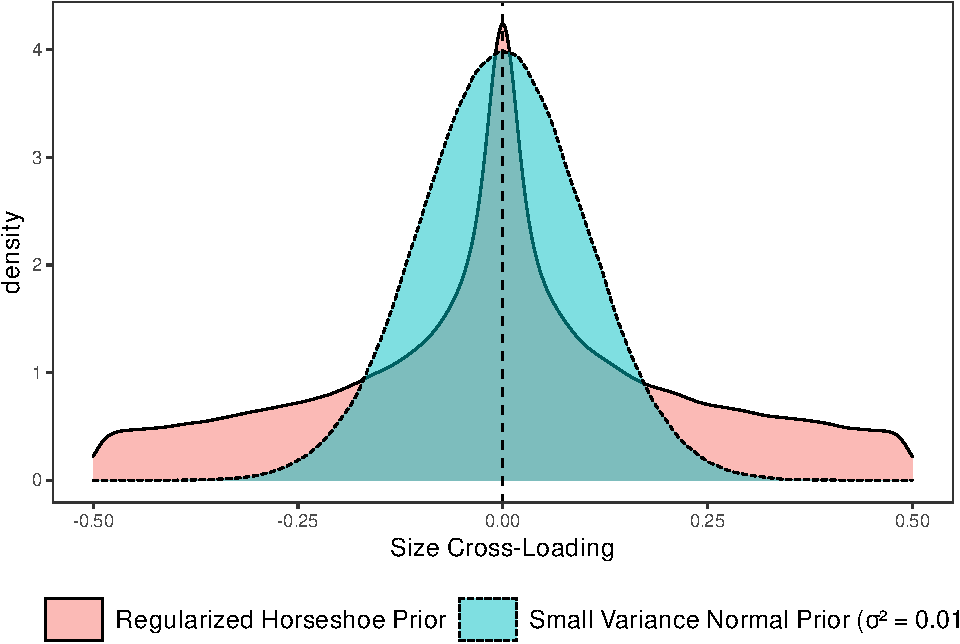
\includegraphics{JMBKoch_report_files/figure-latex/unnamed-chunk-1-1.pdf}
\caption{\label{fig:unnamed-chunk-1}Density Plots of the Regularization Priors of Interest.}
\end{figure}

Figure 1 compares the two shrinkage-priors. Both priors share a large peak at zero, which ensures that cross-loadings are shrunken to(wards) zero. However, the RHSP has much fatter tails. Here, for larger cross-loadings, there is thus much more prior mass than with the SVNP. This ensures that large cross-loadings, that would have been shrunken heavily towards zero with the SVNP, can escape the shrinkage.

\hypertarget{the-current-study}{%
\section{The current study}\label{the-current-study}}

While the Regularized Horseshoe Prior has been shown to perform excellently in the selection of relevant predictors in regression (Piironen \& Vehtari, 2017b; Van Erp et al., 2019), no previous research has validated its performance in selecting relevant cross-loadings in CFA. To fill this gap, we aim to compare the RHSP to the SVNP in their performance in selecting the true factor structure in CFA. Below we present our preliminary results regarding the performance of the SVNP.

\hypertarget{study-procedure-and-parameters}{%
\subsection{Study Procedure and Parameters}\label{study-procedure-and-parameters}}

In order to assess the performance of the SVNP in regularizing cross-loadings in Bayesian Regularized SEM, a Monte Carlo simulation study was conducted using STAN (Stan Development Team, 2021). All code that was used to run the simulation study can be openly accessed on the author's \href{https://github.com/JMBKoch/1vs2StepBayesianRegSEM}{\textbf{github}}\footnote{Specifically, the R-scripts needed to run the simulation can be found on \url{https://github.com/JMBKoch/1vs2StepBayesianRegSEM/tree/main/R}. \texttt{parameters.R} can be adjusted to adjust study parameters, and \texttt{main.R} is used to run the main simulation. Required packages are listed at the top of \texttt{parameters.R}.}. The models were sampled using the No-U-Turn-Sampler (Homan \& Gelman, 2014), with two chains, a burnin-period of 2000 and a chain-length of 4000. These sampling parameters were identified in pilot runs to be required for the RHSP to reach convergence, and were therefore also used for the SVNP in order to ensure a fair comparison.

\hypertarget{true-model-and-conditions}{%
\subsection{True Model and Conditions}\label{true-model-and-conditions}}

The datasets were simulated based on a true 2-factor model, with three items per factor, and a factor correlation of 0.5. The factors were scaled by fixing their means to zero and their variances to 1. All main-loadings were set to 0.75, and all residual variances to 0.3. We included two truly non-zero cross-loadings, that of factor 1 on item 4, and that of factor 2 on item 3. The true model is summarized below, both in equations (Appendix A) and graphically (Figure 2).\footnote{The stan code of the model can be found at \url{https://github.com/JMBKoch/1vs2StepBayesianRegSEM/blob/main/stan/SVNP.stan}.} We varied the magnitude of the two non-zero cross-loadings between 0.2 and 0.5. Next, we varied the sample sizes of the simulated datasets between 100 and 200. This choice was made because for simple factor models researchers would be unlikely to collect larger sample sizes in practice. Finally, based on the recommendations of Muthen and Asparouhov (2012), we included three levels of the hyper-parameter \(\sigma^2\): 0.001, 0.01, 0.1. This left us with a total number of 2 x 2 x 3 = 12 individual sets of conditions. Per set of conditions, 200 replications were run, yielding a total of 2400 replications.

\begin{figure}
\centering
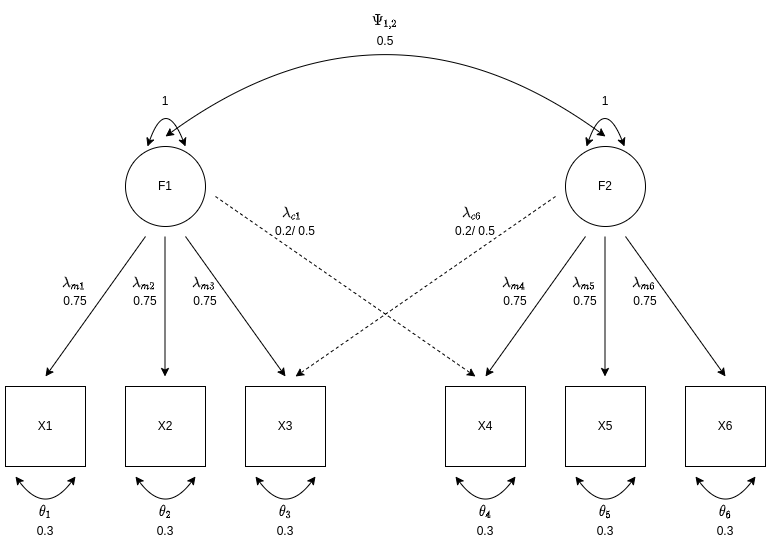
\includegraphics{~/1vs2StepBayesianRegSEM/Rmd/figures/model.png}
\caption{Graphical Representation of the True Model.}
\end{figure}

\hypertarget{outcomes}{%
\subsection{Outcomes}\label{outcomes}}

We focus\footnote{We also computed the Mean Squared Error and Relative Bias of the parameter estimates. The same patterns as with the Mean Absolute Bias emerged. Plots summarizing the findings can be found at \url{https://github.com/JMBKoch/1vs2StepBayesianRegSEM/tree/main/Rmd/plots}.} on the Mean (Absolute) Bias of the posterior mean estimates\footnote{We also computed the outcome based on the median posterior estimates averaged per set of conditions (\(\tilde{\theta}|conditions\)). The results showed no relevant deviations from the mean posterior estimates. See \url{https://github.com/JMBKoch/1vs2StepBayesianRegSEM/tree/main/Rmd/plots/medianEstimates}.} of all model parameters, per set of conditions (\(\bar{\theta} | conditions\)). Hence, for every model parameter \(\theta\) and for every set of conditions that has been sampled from for \(N_{rep}\) replications:
\[Bias_{\bar{\theta} | conditions} = \frac{1}{N} \Sigma_{i = 1}^{N_{rep}} |\bar{\theta_i} - \theta_{true}|\]

\hypertarget{results}{%
\section{Results}\label{results}}

\hypertarget{convergence}{%
\subsection{Convergence}\label{convergence}}

In terms of convergence, the SVNP showed excellent performance. Across all replications and configurations of conditions, there was not a single parameter for which \(\hat{R} > 1.05\). Across all parameters, the minimum value of the Effective Sample Size \(N_{eff}\) was 39.4\% of the chain length, which is a very acceptable proportion. For the largest majority of runs \(N_{eff}\) even exceeded 50\% of the chain length. Moreover, across all runs there was not a single divergent transition. All 2400 replications are therefore included in the results.

\hypertarget{main-results}{%
\subsection{Main Results}\label{main-results}}

The Mean Absolute Bias of all parameters is summarized in Figure 3. For parameter estimates that showed an identical pattern (\(\bar{\lambda}_{c, 2-5}\); \(\bar{\lambda}_{c, 1}\) and \(\bar{\lambda}_{c, 6}\); \(\bar{\lambda}_{m, 1}\), \(\bar{\lambda}_{m, 2}\), \(\bar{\lambda}_{m, 5}\), and \(\bar{\lambda}_{m, 6}\); \(\bar{\lambda}_{m, 3-4}\); and \(\bar{\theta}_{1-6}\)), the first respecting estimate is presented representative for all, both in the plot and in the numbers presented below. The patterns for the two sample size are almost entirely identical, with a tendency for patterns to be slightly more extreme with N = 100. We therefore decided to only present the results for N = 200.\footnote{The Mean Absolute Bias plotted per N can be found on \url{https://github.com/JMBKoch/1vs2StepBayesianRegSEM/blob/main/Rmd/plots/plotsBiasSVNP.html}.}

\begin{figure}
\centering
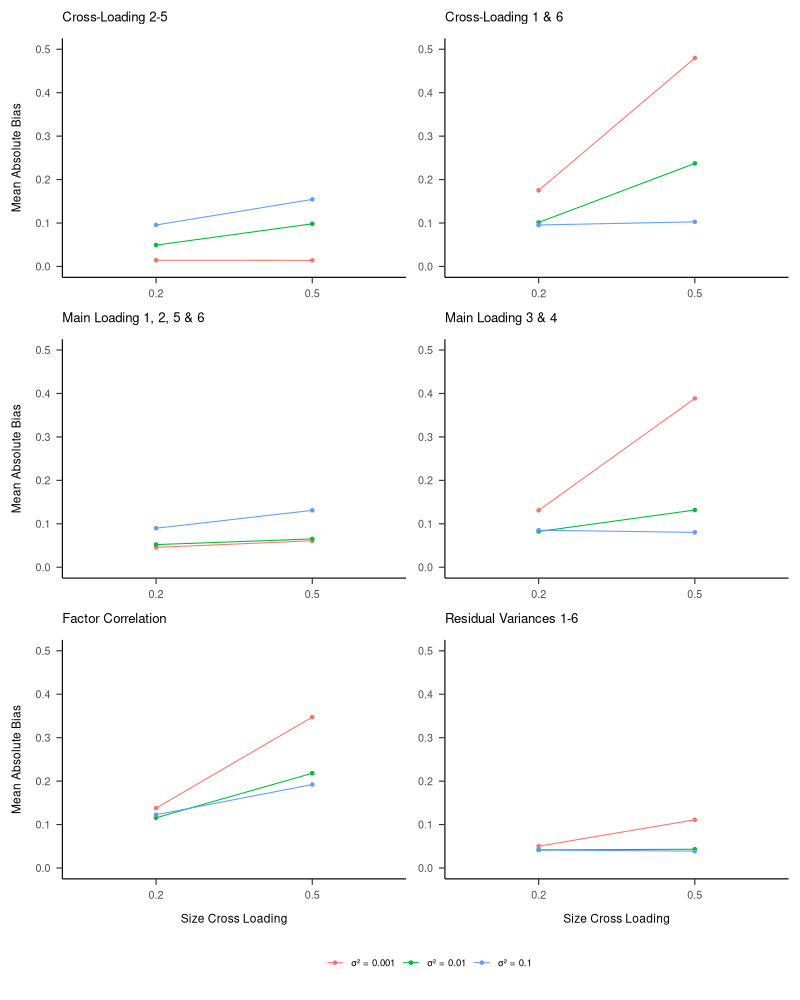
\includegraphics{~/1vs2StepBayesianRegSEM/Rmd/figures/BiasAllPars.png}
\caption{Main Results: Mean Absolute Bias in the Model Parameters (N = 200).}
\end{figure}

Figure 3 shows that, as expected, substantial bias can arise in the model parameters when using the SVNP to regularize cross-loadings. While the bias in the posterior mean estimates of the truly zero cross-loadings \(\bar{\lambda}_{c, 2-5}\) is relatively small, substantial bias arises for the truly non-zero cross-loadings \(\bar{\lambda}_{c, 1}\) and \(\bar{\lambda}_{c, 6}\). Particularly with a large cross-loading of 0.5 and \(\sigma^2 = 0.001\) the bias is substantial, e.g.~\(Bias_{\bar{\lambda}_{c, 1}} = 0.48\), since the true cross-loading of 0.5 is shrunken almost entirely to zero (\(\bar{\lambda}_{c, 1} = 0.02\)). The choice of \(\sigma^2\) plays a crucial role here. Also with \(\sigma^2 = 0.01\) (and true cross-loadings of 0.5) substantial bias still occurs (\(Bias_{\bar{\lambda}_{c, 1}} = 0.24\)). Here the cross-loading is still substantially under-estimated (\(\bar{\lambda}_{c, 1} = 0.26\)), though not entirely shrunken to zero. With a \(\sigma^2 = 0.1\) the bias in the estimate of the cross-loading is less pronounced (\(Bias_{\bar{\lambda}_{c, 1}} = 0.10\)). Here the variance of the prior of the cross-loadings is large enough that the cross-loadings are estimated closer to their large population value, e.g.~\(\bar{\lambda}_{c, 1} = 0.40\).

Next, looking at the main-loadings it is clear that also in the main loadings of factor 1 on item 3 (\(\bar{\lambda}_{m, 3}\)) and of factor 2 on item 4 (\(\bar{\lambda}_{m, 4}\)) substantial bias arises, again in particular under the most extreme combination of conditions. When the true cross-loadings are 0.5 and \(\sigma^2 = 0.001\) the bias becomes very pronounced (e.g.~\(Bias_{\bar{\lambda}_{m, 3}} = 0.39\)). The two loadings have much higher bias than the other four main-loadings as these are the two main-loadings that load onto the same two items on which the truly non-zero cross-loadings load (see Figure 2). When these cross-loadings are shrunken to zero, these main loadings now also have to account for the variance in the items that should be accounted for by the cross-loadings. Consequently, these main-loadings are over-estimated, e.g.~under the above configuration \(\bar{\lambda}_{m, 3} = 1.14\).

Also in the structural parameter of the model, the factor correlation, a similar pattern emerges. While the bias is relatively small and approximately the same for the different values of \(\sigma^2\) when the truly non-zero cross-loadings are 0.2, it becomes more pronounced when they are 0.5, particularly when \(\sigma^2 = 0.001\) (\(Bias_{\bar{r}} = 0.35\)). The underlying pattern becomes clear when considering the posterior mean estimates of the factor correlation. When \(\sigma^2 = 0.001\) and the non-zero cross-loadings are 0.5, the factor correlation is heavily over-estimated (\(\bar{r} = 0.85\)). This is because the covariance between item 3 and 4 that arises from the two cross-loadings, is mis-attributed to the factor-correlation, as the cross-loadings are shrunken to zero.

The bias in the estimates of the residual variances \(\bar{\theta}_{1-6}\) is not substantial across different conditions, although also here a noticeable increase occurs between cross-loadings of 0.2 and 0.5, with \(\sigma^2 = 0.001\).

\hypertarget{conclusions-and-discussion}{%
\section{Conclusions and Discussion}\label{conclusions-and-discussion}}

In sum, a clear pattern arose. The SVNP performs well in situations where the truly non-zero cross-loadings are small, in terms of not leading to extreme bias in the model parameters. However, with larger non-zero cross-loadings, the performance of the SVNP decreases. With smaller values of \(\sigma^2\), particularly with \(\sigma^2 = 0.001\), these cross-loadings are still shrunken to zero, even though they are much larger in practice. This, consequently, causes also substantial bias in main-loadings, and in the factor correlation. In particular the bias in such structural parameters is concerning, as it may lead to highly misleading conclusion in research in which structural relationships between latent constructs are of interest.

Bias occurred much less with \(\sigma^2 = 0.1\). Such relatively large variance still allowed for enough deviations from zero in the cross-loadings to yield relatively accurate estimates of the non-zero cross-loadings itself and consequently the other model parameters. However, this does not mean that one can simply use larger values of \(\sigma^2\) to keep using the SVNP while avoiding bias. In practice, models may include more structural parameters, even more cross-loadings, or a number of residual co-variances. Under these circumstances, large values of \(\sigma^2\) may lead to identification issues. Moreover, the larger \(\sigma^2\), the more cross-loadings will be selected as non-zero, which may ultimately lead to over-fitting.

The RHSP is expected to generally perform better with large non-zero cross-loadings of 0.5, with estimates of these cross-loadings being able to escape the shrinkage. While some hyper-parameter configurations of the RHSP are likely to show much worse performance in terms of identification, other configurations should allow for regularizing cross-loadings without risking substantial bias nor identification issues.

\clearpage

\hypertarget{references}{%
\section{References}\label{references}}

~

\begingroup
\setlength{\parindent}{-0.5in}
\setlength{\leftskip}{0.5in}

\hypertarget{refs}{}
\begin{CSLReferences}{1}{0}
\leavevmode\vadjust pre{\hypertarget{ref-bollen_structural_1989}{}}%
Bollen, K. A. (1989). \emph{Structural {Equations} with {Latent} {Variables}}. John Wiley \& Sons.

\leavevmode\vadjust pre{\hypertarget{ref-carvalho_horseshoe_2010}{}}%
Carvalho, C. M., Polson, N. G., \& Scott, J. G. (2010). The horseshoe estimator for sparse signals. \emph{Biometrika}, \emph{97}(2), 465--480. \url{https://doi.org/10.1093/biomet/asq017}

\leavevmode\vadjust pre{\hypertarget{ref-cox_principles_2006}{}}%
Cox, D. R. (2006). \emph{Principles of {Statistical} {Inference}}. Cambridge University Press.

\leavevmode\vadjust pre{\hypertarget{ref-ghosh_use_2018}{}}%
Ghosh, J., Li, Y., \& Mitra, R. (2018). On the {Use} of {Cauchy} {Prior} {Distributions} for {Bayesian} {Logistic} {Regression}. \emph{Bayesian Analysis}, \emph{13}(2), 359--383. \url{https://doi.org/10.1214/17-BA1051}

\leavevmode\vadjust pre{\hypertarget{ref-hastie_statistical_2015}{}}%
Hastie, T., Tibshirani, R., \& Wainwright, M. (2015). Statistical learning with sparsity. \emph{Monographs on Statistics and Applied Probability}, \emph{143}, 143.

\leavevmode\vadjust pre{\hypertarget{ref-hoerl_ridge_2000}{}}%
Hoerl, A. E., \& Kennard, R. W. (2000). Ridge {Regression}: {Biased} {Estimation} for {Nonorthogonal} {Problems}. \emph{Technometrics}, \emph{42}(1), 80--86. \url{https://doi.org/10.2307/1271436}

\leavevmode\vadjust pre{\hypertarget{ref-homan_no-u-turn_2014}{}}%
Homan, M. D., \& Gelman, A. (2014). The {No}-{U}-turn sampler: Adaptively setting path lengths in {Hamiltonian} {Monte} {Carlo}. \emph{The Journal of Machine Learning Research}, \emph{15}(1), 1593--1623.

\leavevmode\vadjust pre{\hypertarget{ref-hsiang_bayesian_1975}{}}%
Hsiang, T. C. (1975). A {Bayesian} {View} on {Ridge} {Regression}. \emph{Journal of the Royal Statistical Society. Series D (The Statistician)}, \emph{24}(4), 267--268. \url{https://doi.org/10.2307/2987923}

\leavevmode\vadjust pre{\hypertarget{ref-jacobucci_regularized_2016}{}}%
Jacobucci, R., Grimm, K. J., \& McArdle, J. J. (2016). Regularized {Structural} {Equation} {Modeling}. \emph{Structural Equation Modeling: A Multidisciplinary Journal}, \emph{23}(4), 555--566. \url{https://doi.org/10.1080/10705511.2016.1154793}

\leavevmode\vadjust pre{\hypertarget{ref-james_introduction_2021}{}}%
James, G., Witten, D., Hastie, T., \& Tibshirani, R. (2021). \emph{An {Introduction} to {Statistical} {Learning}: With {Applications} in {R}}. New York, NY: Springer US. \url{https://doi.org/10.1007/978-1-0716-1418-1}

\leavevmode\vadjust pre{\hypertarget{ref-lu_bayesian_2016}{}}%
Lu, Z.-H., Chow, S.-M., \& Loken, E. (2016). Bayesian {Factor} {Analysis} as a {Variable}-{Selection} {Problem}: {Alternative} {Priors} and {Consequences}. \emph{Multivariate Behavioral Research}, \emph{51}(4), 519--539. \url{https://doi.org/10.1080/00273171.2016.1168279}

\leavevmode\vadjust pre{\hypertarget{ref-maccallum_model_1992}{}}%
MacCallum, R. C., Roznowski, M., \& Necowitz, L. B. (1992). Model modifications in covariance structure analysis: The problem of capitalization on chance. \emph{Psychological Bulletin}, \emph{111}(3), 490--504. \url{https://doi.org/10.1037/0033-2909.111.3.490}

\leavevmode\vadjust pre{\hypertarget{ref-muthen_bayesian_2012}{}}%
Muthen, B., \& Asparouhov, T. (2012). Bayesian {SEM}: {A} more flexible representation of substantive theory, 78. \url{https://doi.org/10.1037/a0026802}

\leavevmode\vadjust pre{\hypertarget{ref-park_bayesian_2008}{}}%
Park, T., \& Casella, G. (2008). The {Bayesian} {Lasso}. \emph{Journal of the American Statistical Association}, \emph{103}(482), 681--686. \url{https://doi.org/10.1198/016214508000000337}

\leavevmode\vadjust pre{\hypertarget{ref-piironen_hyperprior_2017}{}}%
Piironen, J., \& Vehtari, A. (2017a). On the {Hyperprior} {Choice} for the {Global} {Shrinkage} {Parameter} in the {Horseshoe} {Prior}. In \emph{Proceedings of the 20th {International} {Conference} on {Artificial} {Intelligence} and {Statistics}} (pp. 905--913). PMLR. Retrieved from \url{https://proceedings.mlr.press/v54/piironen17a.html}

\leavevmode\vadjust pre{\hypertarget{ref-piironen_sparsity_2017}{}}%
Piironen, J., \& Vehtari, A. (2017b). Sparsity information and regularization in the horseshoe and other shrinkage priors. \emph{Electronic Journal of Statistics}, \emph{11}(2), 5018--5051. \url{https://doi.org/10.1214/17-EJS1337SI}

\leavevmode\vadjust pre{\hypertarget{ref-stan_development_team_stan_2021}{}}%
Stan Development Team. (2021). Stan {User} {Guide}. Retrieved from \url{https://mc-stan.org/docs/2_27/stan-users-guide-2_27.pdf}

\leavevmode\vadjust pre{\hypertarget{ref-tibshirani_regression_1996}{}}%
Tibshirani, R. (1996). Regression {Shrinkage} and {Selection} {Via} the {Lasso}. \emph{Journal of the Royal Statistical Society: Series B (Methodological)}, \emph{58}(1), 267--288. \url{https://doi.org/10.1111/j.2517-6161.1996.tb02080.x}

\leavevmode\vadjust pre{\hypertarget{ref-van_erp_shrinkage_2019}{}}%
Van Erp, S., Oberski, D. L., \& Mulder, J. (2019). Shrinkage priors for {Bayesian} penalized regression. \emph{Journal of Mathematical Psychology}, \emph{89}, 31--50. \url{https://doi.org/10.1016/j.jmp.2018.12.004}

\end{CSLReferences}

\endgroup

\clearpage

\hypertarget{appendix}{%
\section{Appendix}\label{appendix}}

\hypertarget{appendix-a-true-model}{%
\subsection{Appendix A: True Model}\label{appendix-a-true-model}}

For every individual i in i = 1,\ldots, N:
\[Y_i \sim \mathcal{N}(\mathbf{0}, \Sigma),\] where
\[\Sigma = \Lambda\Psi\Lambda',\]
\[\Lambda = 
    \begin{bmatrix}
    0.75 & 0 \\
    0.75 & 0 \\
    0.75 & 0.2/0.5 \\
    0.2/0.5 & 0.75 \\
    0 & 0.75 \\
    0 & 0.75
    \end{bmatrix},\]
\[\Psi =
    \begin{bmatrix}
     1 & 0.5 \\
     0.5 & 1
    \end{bmatrix}
,\] and
\[\Theta = diag[0.3, 0.3, 0.3, 0.3, 0.3, 0.3].\]


\end{document}
